% Options for packages loaded elsewhere
\PassOptionsToPackage{unicode}{hyperref}
\PassOptionsToPackage{hyphens}{url}
%
\documentclass[
]{article}
\usepackage{lmodern}
\usepackage{amssymb,amsmath}
\usepackage{ifxetex,ifluatex}
\ifnum 0\ifxetex 1\fi\ifluatex 1\fi=0 % if pdftex
  \usepackage[T1]{fontenc}
  \usepackage[utf8]{inputenc}
  \usepackage{textcomp} % provide euro and other symbols
\else % if luatex or xetex
  \usepackage{unicode-math}
  \defaultfontfeatures{Scale=MatchLowercase}
  \defaultfontfeatures[\rmfamily]{Ligatures=TeX,Scale=1}
\fi
% Use upquote if available, for straight quotes in verbatim environments
\IfFileExists{upquote.sty}{\usepackage{upquote}}{}
\IfFileExists{microtype.sty}{% use microtype if available
  \usepackage[]{microtype}
  \UseMicrotypeSet[protrusion]{basicmath} % disable protrusion for tt fonts
}{}
\makeatletter
\@ifundefined{KOMAClassName}{% if non-KOMA class
  \IfFileExists{parskip.sty}{%
    \usepackage{parskip}
  }{% else
    \setlength{\parindent}{0pt}
    \setlength{\parskip}{6pt plus 2pt minus 1pt}}
}{% if KOMA class
  \KOMAoptions{parskip=half}}
\makeatother
\usepackage{xcolor}
\IfFileExists{xurl.sty}{\usepackage{xurl}}{} % add URL line breaks if available
\IfFileExists{bookmark.sty}{\usepackage{bookmark}}{\usepackage{hyperref}}
\hypersetup{
  pdftitle={Organización Industrial},
  pdfauthor={Iván Paredes},
  hidelinks,
  pdfcreator={LaTeX via pandoc}}
\urlstyle{same} % disable monospaced font for URLs
\usepackage[margin=1in]{geometry}
\usepackage{color}
\usepackage{fancyvrb}
\newcommand{\VerbBar}{|}
\newcommand{\VERB}{\Verb[commandchars=\\\{\}]}
\DefineVerbatimEnvironment{Highlighting}{Verbatim}{commandchars=\\\{\}}
% Add ',fontsize=\small' for more characters per line
\usepackage{framed}
\definecolor{shadecolor}{RGB}{248,248,248}
\newenvironment{Shaded}{\begin{snugshade}}{\end{snugshade}}
\newcommand{\AlertTok}[1]{\textcolor[rgb]{0.94,0.16,0.16}{#1}}
\newcommand{\AnnotationTok}[1]{\textcolor[rgb]{0.56,0.35,0.01}{\textbf{\textit{#1}}}}
\newcommand{\AttributeTok}[1]{\textcolor[rgb]{0.77,0.63,0.00}{#1}}
\newcommand{\BaseNTok}[1]{\textcolor[rgb]{0.00,0.00,0.81}{#1}}
\newcommand{\BuiltInTok}[1]{#1}
\newcommand{\CharTok}[1]{\textcolor[rgb]{0.31,0.60,0.02}{#1}}
\newcommand{\CommentTok}[1]{\textcolor[rgb]{0.56,0.35,0.01}{\textit{#1}}}
\newcommand{\CommentVarTok}[1]{\textcolor[rgb]{0.56,0.35,0.01}{\textbf{\textit{#1}}}}
\newcommand{\ConstantTok}[1]{\textcolor[rgb]{0.00,0.00,0.00}{#1}}
\newcommand{\ControlFlowTok}[1]{\textcolor[rgb]{0.13,0.29,0.53}{\textbf{#1}}}
\newcommand{\DataTypeTok}[1]{\textcolor[rgb]{0.13,0.29,0.53}{#1}}
\newcommand{\DecValTok}[1]{\textcolor[rgb]{0.00,0.00,0.81}{#1}}
\newcommand{\DocumentationTok}[1]{\textcolor[rgb]{0.56,0.35,0.01}{\textbf{\textit{#1}}}}
\newcommand{\ErrorTok}[1]{\textcolor[rgb]{0.64,0.00,0.00}{\textbf{#1}}}
\newcommand{\ExtensionTok}[1]{#1}
\newcommand{\FloatTok}[1]{\textcolor[rgb]{0.00,0.00,0.81}{#1}}
\newcommand{\FunctionTok}[1]{\textcolor[rgb]{0.00,0.00,0.00}{#1}}
\newcommand{\ImportTok}[1]{#1}
\newcommand{\InformationTok}[1]{\textcolor[rgb]{0.56,0.35,0.01}{\textbf{\textit{#1}}}}
\newcommand{\KeywordTok}[1]{\textcolor[rgb]{0.13,0.29,0.53}{\textbf{#1}}}
\newcommand{\NormalTok}[1]{#1}
\newcommand{\OperatorTok}[1]{\textcolor[rgb]{0.81,0.36,0.00}{\textbf{#1}}}
\newcommand{\OtherTok}[1]{\textcolor[rgb]{0.56,0.35,0.01}{#1}}
\newcommand{\PreprocessorTok}[1]{\textcolor[rgb]{0.56,0.35,0.01}{\textit{#1}}}
\newcommand{\RegionMarkerTok}[1]{#1}
\newcommand{\SpecialCharTok}[1]{\textcolor[rgb]{0.00,0.00,0.00}{#1}}
\newcommand{\SpecialStringTok}[1]{\textcolor[rgb]{0.31,0.60,0.02}{#1}}
\newcommand{\StringTok}[1]{\textcolor[rgb]{0.31,0.60,0.02}{#1}}
\newcommand{\VariableTok}[1]{\textcolor[rgb]{0.00,0.00,0.00}{#1}}
\newcommand{\VerbatimStringTok}[1]{\textcolor[rgb]{0.31,0.60,0.02}{#1}}
\newcommand{\WarningTok}[1]{\textcolor[rgb]{0.56,0.35,0.01}{\textbf{\textit{#1}}}}
\usepackage{graphicx,grffile}
\makeatletter
\def\maxwidth{\ifdim\Gin@nat@width>\linewidth\linewidth\else\Gin@nat@width\fi}
\def\maxheight{\ifdim\Gin@nat@height>\textheight\textheight\else\Gin@nat@height\fi}
\makeatother
% Scale images if necessary, so that they will not overflow the page
% margins by default, and it is still possible to overwrite the defaults
% using explicit options in \includegraphics[width, height, ...]{}
\setkeys{Gin}{width=\maxwidth,height=\maxheight,keepaspectratio}
% Set default figure placement to htbp
\makeatletter
\def\fps@figure{htbp}
\makeatother
\setlength{\emergencystretch}{3em} % prevent overfull lines
\providecommand{\tightlist}{%
  \setlength{\itemsep}{0pt}\setlength{\parskip}{0pt}}
\setcounter{secnumdepth}{-\maxdimen} % remove section numbering

\title{Organización Industrial}
\author{Iván Paredes}
\date{10/4/2020}

\begin{document}
\maketitle

{
\setcounter{tocdepth}{4}
\tableofcontents
}
\hypertarget{organizaciuxf3n-industrial}{%
\section{Organización Industrial}\label{organizaciuxf3n-industrial}}

La Organización industrial es un campo o área de conocimiento de teoría
de la empresa que trata de los sistemas productivos y de la relación y
límites entre las estructuras de las empresas y los mercados. Trata
asuntos como la competencia perfecta, el costo de las transacciones,
acción de gobierno o dirección.

\hypertarget{historia}{%
\section{Historia}\label{historia}}

Fue Bain (1968) quien sistematizó los aportes realizados por numerosos
autores y estableció el paradigma conocido como:
``Estructura-Conducta-Resultados'' como el elemento básico de análisis y
evaluación de los mercados y para investigar las relaciones entre la
estructura industrial y los resultados obtenidos por el subsector
correspondiente. economía de la información, las barreras de entrada de
nuevas empresas en una situación de competencia imperfecta y monopolio.

El nombre de ``Organización industrial'' y surgieron de Harvard. En
Harvard y en otros lugares, una variedad de descriptivos cursos
institucionales habían aparecido en tales campos como servicios
públicos, fideicomisos, corporaciones, organizaciones financieras n,
agricultura y comercialización. Típicamente, estos cursos no se
integraron con la economía. ({\textbf{???}})\{grether1970industrial\}

\hypertarget{mercados}{%
\section{Mercados}\label{mercados}}

Los mercados permiten a compradores y vendedores intercambiar bienes y
servicios a cambio de un dinero pago. Los mercados vienen en una miríada
de diferentes variedades. Algunos ejemplos son los agricultores locales.

Estos mercados pueden existir en espacio físico o virtual. El análisis
empresarial, la frontera de posibilidades de producción (PPF) es una
curva que ilustra las variaciones en las cantidades que se pueden
producir de dos productos si ambos dependen del mismo recurso finito
para su fabricación.

PPF también juega un papel crucial en la economía. Se puede usar para
demostrar el punto de que la economía de cualquier nación alcanza su
mayor nivel de eficiencia cuando produce solo lo que está mejor
calificado para producir y comercia con otras naciones por el resto de
lo que necesita.

El PPF también se conoce como la curva de posibilidad de producción o la
curva de transformación.

\begin{Shaded}
\begin{Highlighting}[]
\CommentTok{# Graficar una frontera de posibilidades de producción}
\KeywordTok{library}\NormalTok{(}\StringTok{"ggplot2"}\NormalTok{)}
\end{Highlighting}
\end{Shaded}

\begin{verbatim}
## Warning: package 'ggplot2' was built under R version 3.6.3
\end{verbatim}

\begin{Shaded}
\begin{Highlighting}[]
\CommentTok{#Contamos con 10,000 unidades de producción, eso nos permite producir 100 unidades de producto Y o 100 de producto X.}
\NormalTok{eq =}\StringTok{ }\ControlFlowTok{function}\NormalTok{(x)\{(}\DecValTok{10000} \OperatorTok{-}\StringTok{ }\NormalTok{x}\OperatorTok{^}\DecValTok{2}\NormalTok{)}\OperatorTok{^}\NormalTok{(}\DecValTok{1}\OperatorTok{/}\DecValTok{2}\NormalTok{)\}}
\KeywordTok{ggplot}\NormalTok{(}\KeywordTok{data.frame}\NormalTok{(}\DataTypeTok{x=}\KeywordTok{c}\NormalTok{(}\DecValTok{0}\NormalTok{, }\DecValTok{100}\NormalTok{)), }\KeywordTok{aes}\NormalTok{(}\DataTypeTok{x=}\NormalTok{x)) }\OperatorTok{+}\StringTok{ }
\StringTok{  }\KeywordTok{stat_function}\NormalTok{(}\DataTypeTok{fun=}\NormalTok{eq)}
\end{Highlighting}
\end{Shaded}

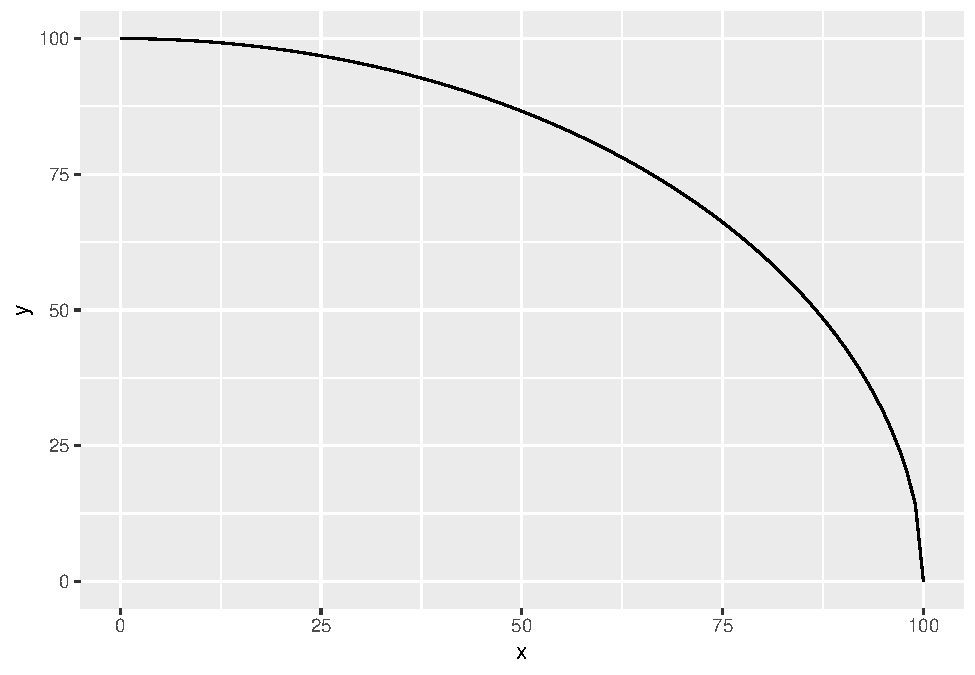
\includegraphics{Orga-Industrial_files/figure-latex/cars-1.pdf}

\begin{Shaded}
\begin{Highlighting}[]
\NormalTok{eq =}\StringTok{ }\ControlFlowTok{function}\NormalTok{(x)\{(}\DecValTok{25} \OperatorTok{-}\StringTok{ }\NormalTok{x}\OperatorTok{^}\DecValTok{2}\NormalTok{)}\OperatorTok{^}\NormalTok{(}\DecValTok{1}\OperatorTok{/}\DecValTok{2}\NormalTok{)\}}
\KeywordTok{ggplot}\NormalTok{(}\KeywordTok{data.frame}\NormalTok{(}\DataTypeTok{x=}\KeywordTok{c}\NormalTok{(}\DecValTok{0}\NormalTok{, }\DecValTok{5}\NormalTok{)), }\KeywordTok{aes}\NormalTok{(}\DataTypeTok{x=}\NormalTok{x)) }\OperatorTok{+}\StringTok{ }
\StringTok{  }\KeywordTok{stat_function}\NormalTok{(}\DataTypeTok{fun=}\NormalTok{eq)}
\end{Highlighting}
\end{Shaded}

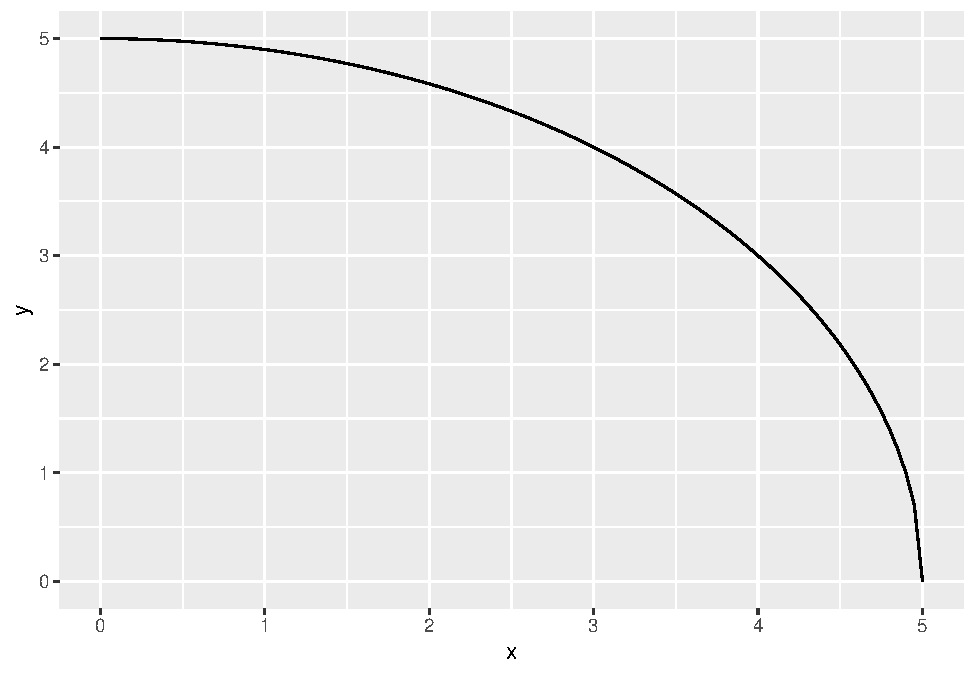
\includegraphics{Orga-Industrial_files/figure-latex/cars-2.pdf}

\hypertarget{empresas-y-consumidores}{%
\section{Empresas y consumidores}\label{empresas-y-consumidores}}

En esta sección, describimos cómo las empresas y los consumidores
generalmente se modelan en la teoría de organización industrial.

\hypertarget{empresas}{%
\subsection{Empresas}\label{empresas}}

Las empresas son esencialmente asociado a un programa de maximización de
ganancias y examinamos el componente de beneficios específicos de la
empresa, es decir, su función de costos. Ingresos totales, el otro
componente de ganancias, dependen de las preferencias de los
consumidores (que determinan la demanda) y del tipo de interacción del
mercado.

\hypertarget{tecnologuxeda}{%
\subsection{Tecnología}\label{tecnologuxeda}}

\hypertarget{tecnologuxeda-cobb-douglas}{%
\subsubsection{tecnología
Cobb-Douglas}\label{tecnologuxeda-cobb-douglas}}

La función Cobb-Douglas es una forma de función de producción,
ampliamente usada para representar las relaciones entre un producto y
las variaciones de los insumos tecnología, trabajo y capital. Fue
propuesta por Knut Wicksell (1851-1926) e investigada con respecto a la
evidencia estadística concreta, por Charles Cobb y Paul Douglas en 1928.

\hypertarget{tecnologuxeda-leontief}{%
\subsubsection{Tecnología Leontief}\label{tecnologuxeda-leontief}}

\hypertarget{la-tasa-tuxe9cnica-de-sustituciuxf3n}{%
\subsubsection{La tasa técnica de
sustitución}\label{la-tasa-tuxe9cnica-de-sustituciuxf3n}}

la tasa marginal de sustitución técnica ( MRTS ), o tasa técnica de
sustitución ( TRS ), es la cantidad en la que debe reducirse la cantidad
de una entrada ( \{~displaystyle - ~Delta x\_ \{2\}\}- ~Delta x\_ \{2\}
) cuando se usa una unidad adicional de otra entrada ( \{~displaystyle
~Delta x\_ \{1\} = 1\}~Delta x\_ \{1\} = 1 ), para que la salida
permanezca constante ( \{~displaystyle y = \{~bar \{y\}\}\}y = \{~bar
\{y\}\} ) \#\#\#\#\# TRS para una tecnología Cobb-Douglas

\hypertarget{la-elasticidad-de-sustituciuxf3n}{%
\subsubsection{La elasticidad de
sustitución}\label{la-elasticidad-de-sustituciuxf3n}}

\hypertarget{la-elasticidad-de-sustituciuxf3n-para-el-programa-cobb-douglas-funciuxf3n-de-ducciuxf3n}{%
\paragraph{La elasticidad de sustitución para el programa Cobb-Douglas
función de
ducción}\label{la-elasticidad-de-sustituciuxf3n-para-el-programa-cobb-douglas-funciuxf3n-de-ducciuxf3n}}

\hypertarget{vuelve-a-escala}{%
\subsubsection{Vuelve a escala}\label{vuelve-a-escala}}

\hypertarget{retornos-a-escala-y-la-tecnologuxeda-cobb-douglas}{%
\paragraph{Retornos a escala y la tecnología
Cobb-Douglas}\label{retornos-a-escala-y-la-tecnologuxeda-cobb-douglas}}

\hypertarget{tecnologuxedas-homoguxe9neas-y-homotuxe9ticas}{%
\subparagraph{Tecnologías homogéneas y
homotéticas}\label{tecnologuxedas-homoguxe9neas-y-homotuxe9ticas}}

\hypertarget{la-funciuxf3n-de-producciuxf3n-ces}{%
\paragraph{La función de producción
CES}\label{la-funciuxf3n-de-producciuxf3n-ces}}

\hypertarget{maximizaciuxf3n-de-ganancias}{%
\subsubsection{2.1 Maximización de
ganancias}\label{maximizaciuxf3n-de-ganancias}}

\hypertarget{la-funciuxf3n-de-ganancias-para-la-tecnologuxeda-cobb-douglas}{%
\paragraph{La función de ganancias para la tecnología
Cobb-Douglas}\label{la-funciuxf3n-de-ganancias-para-la-tecnologuxeda-cobb-douglas}}

\hypertarget{propiedades-de-las-funciones-de-demanda-y-oferta.}{%
\paragraph{2.3 Propiedades de las funciones de demanda y
oferta.}\label{propiedades-de-las-funciones-de-demanda-y-oferta.}}

\hypertarget{estuxe1tica-comparativa-utilizando-las-condiciones-de-primer-orden}{%
\paragraph{2.4 Estática comparativa utilizando las condiciones de primer
orden}\label{estuxe1tica-comparativa-utilizando-las-condiciones-de-primer-orden}}

\hypertarget{funcion-de-beneficios}{%
\subsubsection{FUNCION DE BENEFICIOS}\label{funcion-de-beneficios}}

\hypertarget{los-consumidores}{%
\subsection{Los consumidores}\label{los-consumidores}}

Los consumidores como tomadores de decisiones. Por lo general, suponemos
que los consumidores son racionales en el sentido de que eligen lo que
les gusta mejor. No tratamos situaciones en las que los consumidores
eligen sistemáticamente lo que no está en su mejor interés, dada la
información disponible en el momento en que tienen que tomar su
decisión. Si bien esta suposición se hace ampliamente en los modelos
económicos, puede cuestionarse fácilmente. Ciertamente, los consumidores
cometen errores de vez en cuando. Es posible que quieran obtener un
producto en particular, tome el equivocado del estante por error o haga
un clic incorrecto al realizar un pedido desde un minorista en línea.
Aunque los consumidores tienen la intención de elegir lo que más les
gusta, pueden hacer errores sistemáticos en su toma de decisiones. Los
economistas pueden lidiar con este tipo de error. Tal los errores (que
son idiosincrásicos en la población) conducen a una heterogeneidad ex
post entre consumidores.

\(x^2 + y^2 = z^2\)

\[ x^n + y^n = z^n \]

\hypertarget{maximizaciuxf3n-de-la-utilidad}{%
\subsubsection{Maximización de la
utilidad}\label{maximizaciuxf3n-de-la-utilidad}}

La teoría del comportamiento del consumidor utiliza la ley de la
utilidad marginal decreciente para explicar cómo los consumidores
asignan sus ingresos. El modelo de maximización de la utilidad se basa
en los siguientes supuestos: 1. Se supone que los consumidores son
racionales, tratando de obtener el mayor valor por su dinero.

\begin{enumerate}
\def\labelenumi{\arabic{enumi}.}
\setcounter{enumi}{1}
\item
  Los ingresos de los consumidores son limitados porque sus recursos
  individuales son limitados. Se enfrentan a una restricción
  presupuestaria.
\item
  Los consumidores tienen preferencias claras para diversos bienes y
  servicios, por lo tanto conocen su MU para cada unidad sucesiva del
  producto.
\item
  Cada artículo tiene una etiqueta de precio. Los consumidores deben
  elegir entre productos alternativos con sus ingresos monetarios
  limitados.
\end{enumerate}

\[x \in \mathbb{R}^L_+ \ .\]

\hypertarget{excedente-del-consumidor}{%
\subsubsection{Excedente del
consumidor}\label{excedente-del-consumidor}}

El excedente del consumidor es una medida económica de los beneficios
para el consumidor. El excedente del consumidor ocurre cuando el precio
que los consumidores pagan por un producto o servicio es menor que el
precio que están dispuestos a pagar. Es una medida del beneficio
adicional que reciben los consumidores porque están pagando menos por
algo de lo que estaban dispuestos a pagar.

Un excedente del consumidor ocurre cuando el consumidor está dispuesto a
pagar más por un producto dado que el precio de mercado actual.

\hypertarget{variaciones-compensatorias-y-equivalentes}{%
\paragraph{Variaciones compensatorias y
equivalentes}\label{variaciones-compensatorias-y-equivalentes}}

\hypertarget{utilidad-cuasilineal}{%
\paragraph{Utilidad cuasilineal}\label{utilidad-cuasilineal}}

\hypertarget{utilidad-cuasilineal-y-utilidad-de-muxe9trica-monetaria}{%
\paragraph{Utilidad cuasilineal y utilidad de métrica
monetaria}\label{utilidad-cuasilineal-y-utilidad-de-muxe9trica-monetaria}}

\hypertarget{demanda-de-un-bien-discreto}{%
\subsubsection{Demanda de un bien
discreto}\label{demanda-de-un-bien-discreto}}

\hypertarget{utilidad-de-construcciuxf3n-a-partir-de-la-demanda}{%
\subsubsection{Utilidad de construcción a partir de la
demanda}\label{utilidad-de-construcciuxf3n-a-partir-de-la-demanda}}

\hypertarget{otras-interpretaciones-del-excedente-del-consumidor}{%
\paragraph{Otras interpretaciones del excedente del
consumidor}\label{otras-interpretaciones-del-excedente-del-consumidor}}

\hypertarget{equilibrio}{%
\section{Equilibrio}\label{equilibrio}}

\hypertarget{casos-especiales}{%
\subsection{Casos especiales}\label{casos-especiales}}

\hypertarget{subastas}{%
\subsection{Subastas}\label{subastas}}

Una subasta es un proceso de compra y venta de bienes o servicios. Se
ofera un bien y se oyen ofertas, vendiendo el artículo al mejor postor,
es decir quien hizo la mejor ofera. Existen algunas excepciones a esta
definición. La rama de la teoría económica que se ocupa de los tipos de
subasta y el comportamiento de los participantes en las subastas se
llama teoría de la subastas.

La subasta abierta de precios ascendentes es posiblemente la forma más
común de subasta en uso a lo largo de la historia. Los participantes
ofertan abiertamente uno contra el otro, y cada oferta posterior debe
ser más alta que la oferta anterior. Un subastador puede anunciar los
precios, los licitantes pueden presentar sus ofertas por sí mismos o
hacer que un representante convoque una oferta en su nombre, o las
ofertas pueden presentarse electrónicamente con la oferta actual más
alta mostrada públicamente.

Las subastas se aplicaron y se aplican al comercio en diversos
contextos. Estos contextos son antigüedades , pinturas , objetos de
colección raros, vinos caros, productos básicos , ganado , espectro de
radio , automóviles usados , incluso comercio de emisiones y muchos más.

\hypertarget{clasificaciuxf3n-de-las-subastas}{%
\subsubsection{Clasificación de las
subastas}\label{clasificaciuxf3n-de-las-subastas}}

\hypertarget{diseuxf1o-de-la-subasta}{%
\subsubsection{Diseño de la subasta}\label{diseuxf1o-de-la-subasta}}

\hypertarget{bases-del-concurso}{%
\paragraph{Bases del concurso}\label{bases-del-concurso}}

\end{document}
